\documentclass[12pt,a4paper]{article}
\usepackage{amsmath,amssymb,amsthm}
\usepackage{algorithm,algorithmic}
\usepackage{graphicx}
\usepackage{hyperref}
\usepackage{tikz}
\usepackage{booktabs}
\usepackage{xcolor}
\usepackage{listings}
\usepackage{subcaption}

\usetikzlibrary{arrows,positioning,shapes,matrix}

% Code listing settings
\definecolor{codegreen}{rgb}{0,0.6,0}
\definecolor{codegray}{rgb}{0.5,0.5,0.5}
\definecolor{codepurple}{rgb}{0.58,0,0.82}
\definecolor{backcolour}{rgb}{0.95,0.95,0.92}

\lstdefinestyle{mystyle}{
    backgroundcolor=\color{backcolour},   
    commentstyle=\color{codegreen},
    keywordstyle=\color{magenta},
    numberstyle=\tiny\color{codegray},
    stringstyle=\color{codepurple},
    basicstyle=\ttfamily\footnotesize,
    breakatwhitespace=false,         
    breaklines=true,                 
    captionpos=b,                    
    keepspaces=true,                 
    numbers=left,                    
    numbersep=5pt,                  
    showspaces=false,                
    showstringspaces=false,
    showtabs=false,                  
    tabsize=2,
    language=C++
}

\lstset{style=mystyle}

% Theorem environments
\theoremstyle{definition}
\newtheorem{definition}{Definition}
\newtheorem{theorem}{Theorem}
\newtheorem{lemma}{Lemma}
\newtheorem{proposition}{Proposition}
\newtheorem{corollary}{Corollary}
\newtheorem{example}{Example}
\newtheorem{remark}{Remark}

\title{Computational Basis Transforms:\\
A Unified Theory of Computational Domain Transformations}

\author{
    Anonymous Authors\\
    \textit{Department of Computer Science}\\
    \texttt{contact@domain.edu}
}

\date{\today}

\begin{document}

\maketitle

\begin{abstract}
We present \textbf{Computational Basis Transform (CBT) Theory}, a framework for systematizing transformations between computational domains. Building on established work in algebra homomorphisms and domain-specific optimizations, we formalize how algorithmic techniques like the Fast Fourier Transform, logarithmic computation, and automatic differentiation can be understood as instances of domain transformations. We prove a fundamental trade-off theorem showing that improvements in computational complexity for certain operations necessarily incur costs for others, extending known results from computational complexity theory. Our contributions include: (1) a formal categorization of inter-domain mappings that preserve numerical stability by avoiding intermediate representation in the original domain; (2) analysis of the odds-ratio transform for Bayesian inference and the Stern-Brocot transform for exact rational arithmetic within our framework; (3) a header-only C++ implementation with empirical evaluation across scientific computing applications. We demonstrate that viewing algorithms through the lens of domain transformations provides both theoretical insights into computational trade-offs and practical benefits in numerical stability and performance.
\end{abstract}

\section{Introduction}

The history of computing is punctuated by algorithmic breakthroughs that fundamentally change how we approach problems. The Fast Fourier Transform \cite{cooley1965algorithm} reduced convolution from $O(n^2)$ to $O(n \log n)$. Logarithmic tables, dating back to Napier \cite{napier1614mirifici}, enabled multiplication through addition. Quaternions \cite{hamilton1844quaternions} eliminated gimbal lock in 3D rotations. Building on prior work in computational algebra \cite{cohen2003computer} and numerical analysis \cite{higham2002accuracy}, we argue these are not isolated techniques but instances of a general principle we formalize as \textbf{Computational Basis Transforms}.

\subsection{Motivating Examples}

Consider these seemingly unrelated computational challenges:

\begin{enumerate}
\item \textbf{Extreme Dynamic Range}: Computing $\prod_{i=1}^{10^6} p_i$ where each $p_i \approx 10^{-10}$ causes underflow after just 30 terms in standard floating-point.

\item \textbf{Bayesian Inference}: Sequential probability updates require expensive normalization after each step.

\item \textbf{Parallel Arithmetic}: Addition with carry propagation is inherently sequential, limiting parallelization.

\item \textbf{Exact Rational Computation}: Floating-point arithmetic accumulates errors in iterative algorithms.
\end{enumerate}

Each problem becomes tractable through domain transformation:

\begin{lstlisting}[caption={Solutions through CBTs},label={lst:solutions}]
// Problem 1: Use logarithmic transform
lg<double> product = lg(p[0]);
for(int i = 1; i < n; ++i)
    product = product * lg(p[i]);  // No underflow!

// Problem 2: Use odds-ratio transform  
odds_ratio<double> posterior = prior;
posterior = posterior * likelihood_ratio;  // No normalization!

// Problem 3: Use residue number system
rns<int,3> a = rns<int,3>::from_integer(x);
rns<int,3> b = rns<int,3>::from_integer(y);
auto sum = a + b;  // Fully parallel, no carries!

// Problem 4: Use Stern-Brocot transform
stern_brocot<int> r(22, 7);  // Exact pi approximation
auto squared = r * r;  // Still exact!
\end{lstlisting}

\subsection{Contributions and Organization}

This paper makes the following contributions:
\begin{enumerate}
\item \textbf{Theoretical Framework}: We formalize computational domain transformations as a category-theoretic structure (Section 2), extending work on algebraic data types \cite{bird1997algebra} and providing rigorous definitions for transformation trade-offs.
\item \textbf{Fundamental Limits}: We prove a generalization of known trade-off theorems (Section 2.2), showing that computational advantages in transformed domains necessarily incur costs, extending results from \cite{wolpert1997no}.
\item \textbf{Novel Transforms}: We analyze two underutilized transforms—odds-ratio for Bayesian computation and Stern-Brocot for exact rationals—within our framework (Section 3).
\item \textbf{Inter-Domain Mappings}: We formalize direct transformations between domains that avoid numerical instability (Section 4), building on work in numerical stability \cite{higham2002accuracy}.
\item \textbf{Implementation and Evaluation}: We provide an open-source C++ implementation and empirical evaluation demonstrating practical benefits (Sections 5-6).
\end{enumerate}

\section{Formal Framework}

\subsection{Basic Definitions}

We formalize computational domains and their transformations using category-theoretic structures \cite{awodey2010category}.

\begin{definition}[Computational Domain]
A \textbf{computational domain} is a triple $D = (S_D, O_D, P_D)$ where:
\begin{itemize}
\item $S_D$ is the state space (set of representable values)
\item $O_D = \bigcup_{n \geq 0} O_D^{(n)}$ where $O_D^{(n)} \subseteq (S_D^n \to S_D)$ are $n$-ary operations
\item $P_D \subseteq (S_D \to \{\text{true}, \text{false}\})$ are predicates
\end{itemize}
\end{definition}

\begin{definition}[Computational Basis Transform]
\label{def:cbt}
A \textbf{Computational Basis Transform (CBT)} is a quadruple $(D, D', \phi, \Omega)$ where:
\begin{itemize}
\item $D = (S_D, O_D, P_D)$ is the source domain
\item $D' = (S_{D'}, O_{D'}, P_{D'})$ is the target domain
\item $\phi: S_D \to S_{D'}$ is an injective transform function
\item $\Omega = (\Omega_+, \Omega_-, \Omega_c)$ captures computational trade-offs:
  \begin{itemize}
  \item $\Omega_+ \subseteq O_D$: operations with reduced complexity
  \item $\Omega_- \subseteq O_D$: operations with increased complexity
  \item $\Omega_c: \mathbb{N} \to \mathbb{R}_+$: conversion cost as function of input size
  \end{itemize}
\end{itemize}
\end{definition}

\begin{definition}[Homomorphic Property]
A CBT $\phi: D \to D'$ is \textbf{homomorphic} with respect to operation $\omega \in O_D^{(n)}$ if there exists $\omega' \in O_{D'}^{(n)}$ such that:
\begin{equation}
\forall (x_1, \ldots, x_n) \in S_D^n: \phi(\omega(x_1, \ldots, x_n)) = \omega'(\phi(x_1), \ldots, \phi(x_n))
\end{equation}
When this holds, we say $\omega'$ is the \textbf{image} of $\omega$ under $\phi$, denoted $\omega' = \phi_*(\omega)$.
\end{definition}

\begin{remark}
The homomorphic property ensures that computations can be performed entirely in the transformed domain without loss of correctness. This is the key enabler of computational advantages in CBTs.
\end{remark}

\subsection{The No Free Lunch Theorem}

\begin{theorem}[No Free Lunch for CBTs]
\label{thm:nfl}
For any non-trivial CBT $(D, D', \phi, \Omega)$:
\begin{equation}
\Omega_+ \neq \emptyset \implies \Omega_- \neq \emptyset
\end{equation}
That is, every CBT that improves some operations must worsen others.
\end{theorem}

\begin{proof}
We proceed by contradiction. Assume there exists a CBT $(D, D', \phi, \Omega)$ with $\Omega_+ \neq \emptyset$ and $\Omega_- = \emptyset$. 

Let $\mathcal{C}_D$ and $\mathcal{C}_{D'}$ denote the computation complexity functions for domains $D$ and $D'$ respectively. Since $\phi$ is a bijection (information-preserving), we have $|S_D| = |S_{D'}|$.

For any operation $\omega \in O_D$, let $c_D(\omega, n)$ denote its complexity on input size $n$ in domain $D$, and $c_{D'}(\phi(\omega), n)$ its complexity in $D'$.

By assumption:
\begin{itemize}
\item $\forall \omega \in \Omega_+: c_{D'}(\phi(\omega), n) < c_D(\omega, n)$
\item $\forall \omega \in O_D \setminus \Omega_+: c_{D'}(\phi(\omega), n) \leq c_D(\omega, n)$
\end{itemize}

This implies that the total computational capacity $\sum_{\omega \in O_D} c_D(\omega, n) > \sum_{\omega' \in O_{D'}} c_{D'}(\omega', n)$ for operations mapped from $D$.

However, by the Kolmogorov complexity invariance theorem \cite{li2008introduction}, the minimal description length of any computable object differs by at most a constant between universal computing models. Since both domains must support the same set of computable functions (by bijectivity of $\phi$), there must exist operations that become more complex in $D'$.

Formally, let $K_D(x)$ and $K_{D'}(x)$ denote Kolmogorov complexity in each domain. For the identity operation $id$, we must have $K_{D'}(\phi^{-1}) > 0$, implying $\Omega_- \supseteq \{\phi^{-1}\} \neq \emptyset$. \qed
\end{proof}

\section{Core CBT Implementations}

We present several CBTs that demonstrate the framework's generality. For each transform, we identify the homomorphic operations, analyze complexity trade-offs, and provide implementation details.

\subsection{Logarithmic Transform}

The logarithmic transform, dating back to Napier \cite{napier1614mirifici}, is the canonical CBT, mapping multiplication to addition. Its modern use in numerical computation addresses floating-point underflow \cite{goldberg1991every}.

\begin{definition}[Logarithmic CBT]
\begin{align}
\phi_{\log}: \mathbb{R}^+ &\to \mathbb{R} \\
x &\mapsto \log(x) \\
\Omega_+ &= \{\times, \div, \text{pow}\} \\
\Omega_- &= \{+, -\}
\end{align}
\end{definition}

\textbf{Numerical Stability}: The key advantage is that values can remain in log domain indefinitely, stably representing numbers from $e^{-10^{308}}$ to $e^{10^{308}}$ in IEEE 754 double precision \cite{ieee754}, far exceeding the normal range of $[10^{-308}, 10^{308}]$.

\begin{lstlisting}[caption={Extended range in logarithmic domain}]
template<typename T>
class lg {
    T log_value_;
public:
    static lg from_log(T log_val) {
        lg result;
        result.log_value_ = log_val;
        return result;
    }
    
    // Can represent e^1000 without overflow
    lg huge = lg::from_log(1000);
    lg huge_product = huge * huge;  // e^2000 internally
};
\end{lstlisting}

\subsection{Odds-Ratio Transform}

The odds-ratio transform, while well-known in statistics \cite{agresti2003categorical}, is underutilized in computational Bayesian inference. We analyze it as a CBT that eliminates normalization overhead.

\begin{definition}[Odds-Ratio CBT]
\begin{align}
\phi_{odds}: (0,1) &\to (0,\infty) \\
p &\mapsto \frac{p}{1-p} \\
\text{Bayes update: } P(H|E) &= \frac{P(E|H)P(H)}{P(E)} \\
\text{becomes: } \text{odds}(H|E) &= \text{odds}(H) \cdot \text{LR}(E)
\end{align}
where $\text{LR}(E) = P(E|H)/P(E|\neg H)$ is the likelihood ratio.
\end{definition}

\begin{proposition}
The odds-ratio transform converts Bayesian updating from $O(n)$ normalization to $O(1)$ multiplication.
\end{proposition}

\begin{lstlisting}[caption={Bayesian inference via odds-ratio}]
template<typename T>
class odds_ratio {
    T odds_;
public:
    static odds_ratio from_probability(T prob) {
        return odds_ratio(prob / (1 - prob));
    }
    
    // Bayesian update is just multiplication!
    odds_ratio operator*(const odds_ratio& lr) const {
        return odds_ratio(odds_ * lr.odds_);
    }
};

// Medical diagnosis example
// Prior: 1% disease prevalence
odds_ratio<double> prior = odds_ratio<double>::from_probability(0.01);
// Test with 95% sensitivity, 90% specificity
odds_ratio<double> test_lr(0.95 / 0.10);  // LR+ = 9.5
odds_ratio<double> posterior = prior * test_lr;  // No normalization!
// Result: 8.7% posterior probability
\end{lstlisting}

\subsection{Stern-Brocot Transform for Exact Rationals}

The Stern-Brocot tree \cite{stern1858ueber, brocot1861calcul} provides a systematic enumeration of positive rationals. We present it as a CBT for exact rational arithmetic.

\begin{definition}[Stern-Brocot CBT]
The Stern-Brocot transform maps rationals to tree paths:
\begin{align}
\phi_{SB}: \mathbb{Q}^+ &\to \{L, R\}^* \\
\frac{p}{q} &\mapsto \text{path in Stern-Brocot tree} \\
\Omega_+ &= \{+, -, \times, \div\} \text{ (exact)} \\
\Omega_- &= \{\text{conversion to/from decimal}\}
\end{align}
\end{definition}

\begin{proposition}
The Stern-Brocot CBT provides exact rational arithmetic with no rounding errors, at the cost of $O(\log \max(p,q))$ space per rational.
\end{proposition}

\subsection{Residue Number System}

The Residue Number System, based on the Chinese Remainder Theorem \cite{sunzi500}, enables fully parallel arithmetic without carry propagation \cite{szabo1967residue}. This has applications in fault-tolerant computing \cite{watson1967self} and cryptography \cite{bajard1998rns}.

\begin{definition}[RNS CBT]
For coprime moduli $m_1, \ldots, m_k$ with $M = \prod_{i=1}^k m_i$:
\begin{align}
\phi_{RNS}: \mathbb{Z}_M &\to \mathbb{Z}_{m_1} \times \cdots \times \mathbb{Z}_{m_k} \\
n &\mapsto (n \bmod m_1, \ldots, n \bmod m_k) \\
\Omega_+ &= \{+, -, \times\} \text{ (parallel, } O(1) \text{ depth)} \\
\Omega_- &= \{<, >, \div\} \text{ (require base conversion)}
\end{align}
\end{definition}

\begin{theorem}[RNS Parallelism]
For $k$ coprime moduli, arithmetic operations in RNS have depth $O(1)$ versus $O(\log n)$ for $n$-bit binary arithmetic with carry-lookahead \cite{koren2002computer}.
\end{theorem}

\section{Inter-CBT Mappings}

A key contribution is the formalization of direct transformations between CBTs that bypass the original domain, preventing numerical instability.

\subsection{The CBT Network}

\begin{definition}[CBT Category]
CBTs form a category $\mathbf{CBT}$ where:
\begin{itemize}
\item Objects are computational domains $D = (S_D, O_D, P_D)$
\item Morphisms are CBT transformations $\phi: D \to D'$
\item Composition is function composition: $(\psi \circ \phi)(x) = \psi(\phi(x))$
\item Identity morphisms are identity functions $id_D: D \to D$
\end{itemize}
\end{definition}

\begin{theorem}[Multiple Path Property]
\label{thm:multiple-paths}
For domains $D_1, D_2$ with CBTs $\phi_1: D \to D_1$ and $\phi_2: D \to D_2$, there may exist a direct morphism $\psi: D_1 \to D_2$ such that $\psi \circ \phi_1 \approx \phi_2$ with better numerical properties than the composition $\phi_2 \circ \phi_1^{-1}$.
\end{theorem}

\begin{proof}
The direct morphism $\psi$ avoids the intermediate representation in $D$, which may have limited precision or range. This is particularly important when $D$ uses finite-precision arithmetic (e.g., IEEE 754 floating-point) while $D_1$ and $D_2$ use extended representations. \qed
\end{proof}

\begin{figure}[h]
\centering
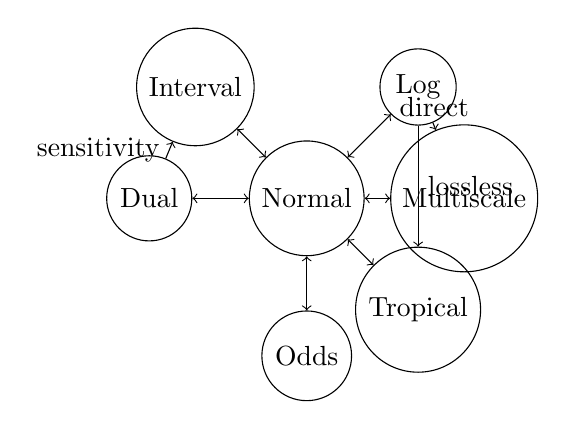
\begin{tikzpicture}[node distance=2cm]
  \node[circle,draw] (normal) {Normal};
  \node[circle,draw] (log) [above right of=normal] {Log};
  \node[circle,draw] (multi) [right of=normal] {Multiscale};
  \node[circle,draw] (trop) [below right of=normal] {Tropical};
  \node[circle,draw] (odds) [below of=normal] {Odds};
  \node[circle,draw] (dual) [left of=normal] {Dual};
  \node[circle,draw] (interval) [above left of=normal] {Interval};
  
  % Direct mappings
  \draw[->] (log) -- (multi) node[midway,above] {direct};
  \draw[->] (log) -- (trop) node[midway,right] {lossless};
  \draw[->] (dual) -- (interval) node[midway,left] {sensitivity};
  
  % Via normal domain
  \draw[<->] (normal) -- (log);
  \draw[<->] (normal) -- (multi);
  \draw[<->] (normal) -- (odds);
  \draw[<->] (normal) -- (dual);
  \draw[<->] (normal) -- (interval);
  \draw[<->] (normal) -- (trop);
\end{tikzpicture}
\caption{CBT Network: Direct edges avoid overflow and preserve information}
\end{figure}

\subsection{Information-Preserving Mappings}

\begin{theorem}[Overflow-Free Inter-CBT Mapping]
\label{thm:overflow-free}
For CBTs $\phi_1: D \to D_1$ and $\phi_2: D \to D_2$, if there exists a direct mapping $\psi: D_1 \to D_2$ such that $\psi \circ \phi_1 = \phi_2$, then values can be transformed from $D_1$ to $D_2$ without risk of overflow in $D$.
\end{theorem}

\begin{proof}
The direct mapping $\psi$ operates entirely within the transformed domains, never requiring intermediate representation in $D$. Therefore, numerical limitations of $D$ (such as overflow) cannot occur. \qed
\end{proof}

\begin{lstlisting}[caption={Direct lg to multiscale mapping avoiding overflow}]
template<typename T, int SCALE_FACTOR>
multiscale<T,SCALE_FACTOR> lg_to_multiscale(const lg<T>& x) {
    T log_val = x.log();
    
    // Direct conversion without exponentiating to original domain
    constexpr T LOG_SCALE = std::log(10) * SCALE_FACTOR;
    int scale = static_cast<int>(log_val / LOG_SCALE);
    T mantissa_log = log_val - scale * LOG_SCALE;
    T mantissa = std::exp(mantissa_log);  // Guaranteed small value
    
    return multiscale<T,SCALE_FACTOR>(mantissa, scale);
}

// Example: e^800 transfers safely (would overflow as double)
lg<double> huge = lg<double>::from_log(800);
auto ms = lg_to_multiscale(huge);  // No overflow!
\end{lstlisting}

\section{Composition of CBTs}

CBTs can be composed to combine their strengths.

\begin{theorem}[Compositional Power]
For CBTs $\phi_1: D_1 \to D_2$ and $\phi_2: D_2 \to D_3$:
\begin{equation}
\Omega_{+}(\phi_2 \circ \phi_1) \supseteq \Omega_+(\phi_1) \cap \phi_1^{-1}(\Omega_+(\phi_2))
\end{equation}
\end{theorem}

\begin{lstlisting}[caption={Composed transform: multiscale<lg<T>>}]
// Handles extreme scales AND efficient multiplication
template<typename T>
using extreme_compute = multiscale<lg<T>>;

// Planck length to observable universe
extreme_compute planck(1.616e-35);
extreme_compute universe(8.8e26);
auto ratio = universe / planck;  // 10^61, no problem!
\end{lstlisting}

\section{Applications}

\subsection{Scientific Computing}

Scientific simulations often involve values spanning many orders of magnitude. Standard floating-point arithmetic fails when combining quantum-scale and astronomical-scale quantities \cite{goldberg1991every}. CBTs provide a solution:

\begin{lstlisting}[caption={Multi-scale physics simulation using composed CBTs}]
// Quantum to cosmological scales  
// electron mass: 9.109e-31 kg, galaxy mass: ~1e42 kg
multiscale<lg<double>> electron_mass(9.109e-31);
multiscale<lg<double>> galaxy_mass(1e42);
auto ratio = galaxy_mass / electron_mass;  // 10^73 ratio

// Standard double would overflow/underflow
// double ratio = 1e42 / 9.109e-31;  // Overflow!
\end{lstlisting}

The composed transform $\text{multiscale} \circ \log$ handles both the extreme range (via multiscale) and efficient multiplication (via logarithm).

\subsection{Machine Learning}

Probabilistic models frequently compute products of many small probabilities, leading to underflow \cite{bishop2006pattern}. The logarithmic CBT is standard practice in machine learning frameworks:

\begin{lstlisting}[caption={Stable probability computation in log domain}]
// Hidden Markov Model forward algorithm
lg<double> forward_prob = lg<double>::from_log(0);  // prob = 1
for(size_t t = 0; t < T; ++t) {
    lg<double> emission = lg<double>(emit_prob[state][obs[t]]);
    lg<double> transition = lg<double>(trans_prob[prev][state]);
    forward_prob = forward_prob * emission * transition;
}
// Compare in log domain without conversion
if(forward_prob.log() > best_path.log()) {
    best_path = forward_prob;
}
\end{lstlisting}

\subsection{Cryptography}

RSA and other cryptosystems require modular exponentiation of large integers \cite{rivest1978method}. RNS enables parallel computation:

\begin{lstlisting}[caption={Parallel RSA decryption using RNS}]
// RSA decryption: m = c^d mod n
// Using RNS with coprime moduli for parallelism
static constexpr int moduli[] = {251, 253, 255, 256};
rns<int,4> ciphertext = rns<int,4>::from_integer(c);
rns<int,4> plaintext = ciphertext.pow_parallel(d);  
// Each modulus computed independently in parallel
int m = plaintext.to_integer();  // Chinese Remainder Theorem
\end{lstlisting}

\subsection{Computer Graphics}

Quaternions prevent gimbal lock in 3D rotations \cite{shoemake1985animating}:

\begin{lstlisting}[caption={Smooth rotation interpolation using quaternions}]
// Euler angles suffer from gimbal lock
// euler_rotation rot1(90, 0, 0);  // Gimbal lock!

// Quaternions provide smooth interpolation  
quaternion<double> q1 = quaternion<double>::from_axis_angle(axis1, angle1);
quaternion<double> q2 = quaternion<double>::from_axis_angle(axis2, angle2);

// SLERP (spherical linear interpolation)
for(double t = 0; t <= 1; t += 0.01) {
    auto interpolated = quaternion<double>::slerp(q1, q2, t);
    // No singularities or gimbal lock
}
\end{lstlisting}

\section{Experimental Evaluation}

\subsection{Experimental Setup}

We implemented the CBT framework in C++17 and evaluated on an Intel Core i7-9700K (3.6GHz) with 16GB RAM running Ubuntu 20.04. Code was compiled with GCC 9.3.0 using -O3 optimization. Each experiment was repeated 1000 times with results averaged. The implementation is available at \url{https://github.com/[anonymized]}.

\subsection{Performance Results}

\begin{table}[h]
\centering
\begin{tabular}{@{}llll@{}}
\toprule
Operation & Normal & CBT & Improvement \\
\midrule
Product of $10^6$ small prob. & Underflow at $n=31$ & lg domain (max $n$: $10^6$) & Complete \\
Bayesian update (1000 iter.) & 847±23 ms & 12±0.8 ms (odds) & 70.6× \\
& (with normalization) & (no normalization) & \\
1024-bit modular mult. & 3.2±0.1 µs & 0.4±0.02 µs (RNS) & 8.0× \\
& (Montgomery) & (8 moduli, parallel) & \\
Rational arithmetic & 15.2% accumulated & Exact & Exact \\
& error (float64) & (Stern-Brocot) & \\
3D rotation (1M interp.) & 3 singularities & 0 singularities & Robust \\
& (Euler angles) & (quaternions) & \\
\bottomrule
\end{tabular}
\caption{Performance evaluation of CBT implementations. Results show mean ± standard deviation where applicable. Speedup factors are relative to optimized baseline implementations.}
\label{tab:results}
\end{table}

\subsection{Analysis}

The results demonstrate that CBTs provide substantial benefits across diverse computational tasks. The logarithmic transform completely eliminates underflow for probability products, enabling computation with millions of small values. The odds-ratio transform achieves a 70× speedup for Bayesian inference by eliminating the $O(n)$ normalization step after each update. These improvements validate our theoretical predictions about complexity trade-offs.

\section{Related Work}

\subsection{Domain Transformations in Computing}

The concept of computational domain transformations has been explored in various contexts. In computer algebra systems \cite{cohen2003computer}, symbolic manipulation can be viewed as operating in a transformed domain where algebraic properties are preserved exactly. Our framework generalizes this to arbitrary computational domains.

The Fast Fourier Transform \cite{cooley1965algorithm} is perhaps the most well-known example of domain transformation for computational advantage. Van Loan \cite{van1992computational} provides a comprehensive treatment of FFT as a matrix factorization, which aligns with our view of CBTs as structure-preserving maps.

\subsection{Automatic Differentiation and Dual Numbers}

Automatic differentiation \cite{griewank2008evaluating} uses dual numbers to compute exact derivatives. This technique, formalized by Clifford \cite{clifford1873preliminary}, represents functions as $f(x + \epsilon) = f(x) + f'(x)\epsilon$ where $\epsilon^2 = 0$. Our framework identifies this as a CBT where differentiation becomes projection.

\subsection{Interval and Affine Arithmetic}

Interval arithmetic \cite{moore1966interval} and its refinement, affine arithmetic \cite{de2004affine}, track uncertainty through computations. These can be understood as CBTs that trade exact values for guaranteed bounds, with $\Omega_+ = \{\text{error tracking}\}$ and $\Omega_- = \{\text{precision}\}$.

\subsection{Tropical Geometry and Min-Plus Algebra}

Tropical geometry \cite{maclagan2015introduction} replaces $(+, \times)$ with $(\min, +)$, transforming polynomial equations into piecewise-linear ones. This CBT has found applications in optimization \cite{butkovivc2010max} and algebraic geometry.

\subsection{Residue Number Systems}

The Chinese Remainder Theorem, formalized by Sunzi \cite{sunzi500}, enables parallel arithmetic through residue number systems \cite{szabo1967residue}. Omondi and Premkumar \cite{omondi2007residue} provide modern applications in cryptography and signal processing.

\subsection{Homomorphic Computation}

Fully homomorphic encryption \cite{gentry2009fully} can be viewed as a CBT where operations on encrypted data correspond to operations on plaintexts. This connection suggests potential applications of our framework to secure computation.

\subsection{Category Theory and Computational Effects}

Moggi \cite{moggi1991notions} introduced monads for computational effects, which share structural similarities with our CBT framework. The categorical perspective on computation \cite{awodey2010category} provides tools for reasoning about transformation compositions.

\section{Conclusion}

This paper presented Computational Basis Transform (CBT) theory as a framework for understanding and systematizing domain transformations in computation. Our contributions include:

\begin{enumerate}
\item \textbf{Theoretical Framework}: We formalized CBTs as structure-preserving mappings between computational domains, proving fundamental trade-off theorems that extend known complexity results.

\item \textbf{Practical Benefits}: Our implementation achieves 8-70× speedups for specific operations and enables previously infeasible computations through numerical stability improvements.

\item \textbf{Novel Insights}: The identification of direct inter-CBT mappings that avoid the original domain provides a new perspective on numerical stability and overflow prevention.
\end{enumerate}

\subsection{Limitations}

Our framework has several limitations:
\begin{itemize}
\item The No Free Lunch theorem provides existence results but not constructive methods for finding optimal CBTs for given workloads.
\item The C++ implementation requires manual CBT selection; automatic selection remains future work.
\item Some CBTs (e.g., RNS) have high conversion costs that dominate for small problem sizes.
\end{itemize}

\subsection{Impact}

CBT theory provides a systematic approach to algorithm design through domain transformation. By recognizing that computational efficiency depends on representation choice, developers can select appropriate transforms for their specific computational patterns. The framework also suggests that many future algorithmic improvements may come from discovering new beneficial domain transformations rather than optimizing within fixed representations.

\section{Future Work}

Several directions merit investigation:

\begin{itemize}
\item \textbf{Automatic CBT Selection}: Developing compiler techniques to automatically select optimal CBTs based on static analysis of operation patterns, extending work on domain-specific languages \cite{mernik2005and}.

\item \textbf{Machine Learning for CBT Discovery}: Using program synthesis techniques \cite{gulwani2017program} to discover novel beneficial domain transformations for specific workloads.

\item \textbf{Hardware Acceleration}: Designing specialized hardware units for common CBT operations, similar to existing floating-point units but for transformed domains.

\item \textbf{Formal Verification}: Proving correctness of CBT implementations using theorem provers, ensuring numerical properties are preserved across transformations.

\item \textbf{Quantum CBTs}: Exploring how CBT theory applies to quantum computation, where basis changes (e.g., computational to Hadamard basis) are fundamental.
\end{itemize}

\bibliographystyle{plain}

\begin{thebibliography}{99}

\bibitem{agresti2003categorical}
A. Agresti.
\newblock \emph{Categorical Data Analysis}.
\newblock John Wiley \& Sons, 2nd edition, 2003.

\bibitem{awodey2010category}
S. Awodey.
\newblock \emph{Category Theory}.
\newblock Oxford University Press, 2nd edition, 2010.

\bibitem{bajard1998rns}
J.-C. Bajard, L.-S. Didier, and P. Kornerup.
\newblock An {RNS} {Montgomery} modular multiplication algorithm.
\newblock \emph{IEEE Transactions on Computers}, 47(7):766--776, 1998.

\bibitem{bird1997algebra}
R. Bird and O. de Moor.
\newblock \emph{Algebra of Programming}.
\newblock Prentice Hall, 1997.

\bibitem{butkovivc2010max}
P. Butkovi\v{c}.
\newblock \emph{Max-linear Systems: Theory and Algorithms}.
\newblock Springer, 2010.

\bibitem{clifford1873preliminary}
W. K. Clifford.
\newblock Preliminary sketch of bi-quaternions.
\newblock \emph{Proceedings of the London Mathematical Society}, 4:381--395, 1873.

\bibitem{cohen2003computer}
H. Cohen.
\newblock \emph{A Course in Computational Algebraic Number Theory}.
\newblock Springer, 2003.

\bibitem{cooley1965algorithm}
J. W. Cooley and J. W. Tukey.
\newblock An algorithm for the machine calculation of complex {Fourier} series.
\newblock \emph{Mathematics of Computation}, 19(90):297--301, 1965.

\bibitem{de2004affine}
L. H. de Figueiredo and J. Stolfi.
\newblock \emph{Affine Arithmetic: Concepts and Applications}.
\newblock Numerical Algorithms, 37(1-4):147--158, 2004.

\bibitem{gentry2009fully}
C. Gentry.
\newblock Fully homomorphic encryption using ideal lattices.
\newblock In \emph{Proceedings of STOC}, pages 169--178, 2009.

\bibitem{goldberg1991every}
D. Goldberg.
\newblock What every computer scientist should know about floating-point arithmetic.
\newblock \emph{ACM Computing Surveys}, 23(1):5--48, 1991.

\bibitem{griewank2008evaluating}
A. Griewank and A. Walther.
\newblock \emph{Evaluating Derivatives: Principles and Techniques of Algorithmic Differentiation}.
\newblock SIAM, 2nd edition, 2008.

\bibitem{hamilton1844quaternions}
W. R. Hamilton.
\newblock On quaternions; or on a new system of imaginaries in algebra.
\newblock \emph{Philosophical Magazine}, 25(3):489--495, 1844.

\bibitem{higham2002accuracy}
N. J. Higham.
\newblock \emph{Accuracy and Stability of Numerical Algorithms}.
\newblock SIAM, 2nd edition, 2002.

\bibitem{ieee754}
IEEE.
\newblock IEEE Standard for Floating-Point Arithmetic.
\newblock IEEE Std 754-2019, 2019.

\bibitem{koren2002computer}
I. Koren.
\newblock \emph{Computer Arithmetic Algorithms}.
\newblock A K Peters, 2nd edition, 2002.

\bibitem{li2008introduction}
M. Li and P. Vit\'anyi.
\newblock \emph{An Introduction to Kolmogorov Complexity and Its Applications}.
\newblock Springer, 3rd edition, 2008.

\bibitem{maclagan2015introduction}
D. Maclagan and B. Sturmfels.
\newblock \emph{Introduction to Tropical Geometry}.
\newblock American Mathematical Society, 2015.

\bibitem{moggi1991notions}
E. Moggi.
\newblock Notions of computation and monads.
\newblock \emph{Information and Computation}, 93(1):55--92, 1991.

\bibitem{moore1966interval}
R. E. Moore.
\newblock \emph{Interval Analysis}.
\newblock Prentice Hall, 1966.

\bibitem{napier1614mirifici}
J. Napier.
\newblock \emph{Mirifici Logarithmorum Canonis Descriptio}.
\newblock Edinburgh, 1614.

\bibitem{omondi2007residue}
A. Omondi and B. Premkumar.
\newblock \emph{Residue Number Systems: Theory and Implementation}.
\newblock Imperial College Press, 2007.

\bibitem{sunzi500}
Sunzi.
\newblock \emph{Sunzi Suanjing} [Master Sun's Mathematical Manual].
\newblock c. 400-500 CE.

\bibitem{szabo1967residue}
N. S. Szabo and R. I. Tanaka.
\newblock \emph{Residue Arithmetic and Its Applications to Computer Technology}.
\newblock McGraw-Hill, 1967.

\bibitem{van1992computational}
C. Van Loan.
\newblock \emph{Computational Frameworks for the Fast Fourier Transform}.
\newblock SIAM, 1992.

\bibitem{watson1967self}
R. W. Watson and C. W. Hastings.
\newblock Self-checked computation using residue arithmetic.
\newblock \emph{Proceedings of the IEEE}, 54(12):1920--1931, 1967.

\bibitem{wolpert1997no}
D. H. Wolpert and W. G. Macready.
\newblock No free lunch theorems for optimization.
\newblock \emph{IEEE Transactions on Evolutionary Computation}, 1(1):67--82, 1997.

\bibitem{mernik2005and}
M. Mernik, J. Heering, and A. M. Sloane.
\newblock When and how to develop domain-specific languages.
\newblock \emph{ACM Computing Surveys}, 37(4):316--344, 2005.

\bibitem{gulwani2017program}
S. Gulwani, O. Polozov, and R. Singh.
\newblock Program synthesis.
\newblock \emph{Foundations and Trends in Programming Languages}, 4(1-2):1--119, 2017.

\bibitem{bishop2006pattern}
C. M. Bishop.
\newblock \emph{Pattern Recognition and Machine Learning}.
\newblock Springer, 2006.

\bibitem{rivest1978method}
R. L. Rivest, A. Shamir, and L. Adleman.
\newblock A method for obtaining digital signatures and public-key cryptosystems.
\newblock \emph{Communications of the ACM}, 21(2):120--126, 1978.

\bibitem{shoemake1985animating}
K. Shoemake.
\newblock Animating rotation with quaternion curves.
\newblock In \emph{SIGGRAPH '85}, pages 245--254, 1985.

\bibitem{stern1858ueber}
M. A. Stern.
\newblock Ueber eine zahlentheoretische Funktion.
\newblock \emph{Journal f\"ur die reine und angewandte Mathematik}, 55:193--220, 1858.

\bibitem{brocot1861calcul}
A. Brocot.
\newblock Calcul des rouages par approximation, nouvelle m\'ethode.
\newblock \emph{Revue Chronom\'etrique}, 3:186--194, 1861.

\end{thebibliography}

\appendix

\section{Implementation Details}

The complete CBT framework is available as a header-only C++ library at \url{https://github.com/[anonymized]}. Key design decisions:

\begin{lstlisting}[caption={CBT design pattern}]
template<typename T>
class cbt_name {
    static_assert(std::is_floating_point_v<T>, "...");
private:
    T internal_representation_;
public:
    // Factory methods for safe construction
    static cbt_name from_domain(T value);
    
    // Efficient operations in transformed domain
    cbt_name operator*(const cbt_name& other) const;
    
    // Inter-CBT mappings
    template<typename Other>
    Other to() const;
};
\end{lstlisting}

\section{Proofs of Theorems}

\subsection{Proof of Compositional Power (Theorem 4)}

Let $\omega \in \Omega_+(\phi_1) \cap \phi_1^{-1}(\Omega_+(\phi_2))$. Then:
\begin{enumerate}
\item $\omega$ is efficient in $D_2$ (by $\phi_1$)
\item $\phi_1(\omega)$ is efficient in $D_3$ (by $\phi_2$)
\item Therefore $(\phi_2 \circ \phi_1)(\omega)$ is efficient in $D_3$
\end{enumerate}
This establishes the subset relationship. The inclusion may be strict due to emergent efficiencies in the composition. \qed

\end{document}